\section{Algunas distribuciones de una variable aleatoria}
De forma intuitiva, una variable aleatoria puede concebirse como un valor numérico que está afectado por el azar. Por ejemplo, en una epidemia de alguna enfermedad, se sabe que una persona cualquiera puede enfermar o no (estos serían los sucesos), pero no se sabe con antelación cuál va a ocurrir, solo se puede afirmar que existe una probabilidad de que una persona enferme y otra, de que no. Dependiendo de las circunstancias, estos sucesos no siempre serán equiprobables.\\
Para trabajar de manera sólida con variables aleatorias en general es necesario considerar un gran número de experimentos, para su tratamiento estadístico, cuantificar los resultados de modo que se asigne un número real a cada uno de los resultados posibles del experimento, por lo cual será necesario definir ciertas funciones reales asociadas a una variable aleatoria.
\\\\
Consideremos el caso discreto. Sea $X$ una variable aleatoria discreta que toma los valores $x_0,x_1,x_2,\ldots$ con probabilidades
$$p_0=P(X=x_0)$$
$$p_1=P(X=x_1)$$
$$p_2=P(X=x_2)$$
$$\vdots$$
Esta lista de valores numéricos y sus probabilidades puede ser finita o infinita, pero numerable. La función de probabilidad de $X$ se definiría como aquella función que toma estas probabilidades como valores.
\begin{Def}
    Sea $X$ una variable aleatoria discreta que toma valores sobre un conjunto finito $S$, P la probabilidad inducida por la variable aleatoria $X$. La función de probabilidad de $X$ es una función  $f_{X}:\R\rightarrow\R$ que se define como
    \begin{eqnarray*}
        f_{X}(x)=
        \begin{cases}
            P(X=x) &\textit{Si }x\in S\\0 &\textit{en otro caso}\label{def-funcionProbabilidad}
        \end{cases}
    \end{eqnarray*}
\end{Def}
\begin{Def}
%%%%%% DISTRIBUCIÓN DE POISSON %%%%%%%%%%%%%%%
\label{def-distribuciónProb}
    Al conjunto $\{f(x): x\in S\}$ o $\{P(X=x): x\in S\} $se le conoce como distribución de probabilidad.
\end{Def}
Para hallar la probabilidad de algún evento $B\subset\R$ numerable con variable aleatoria discreta asociada $X$,
$$P(B)=P\big(X\in B)=P\big(\bigcup_{x\in B}(X=x)\big)=\sum_{x\in B}P(X=x)=\sum_{x\in B}f_X(x)$$
De esta manera que la función de probabilidad $f_X$ muestra la forma en que la probabilidad se distribuye sobre un conjunto discreto. Si $f$ es una función de probabilidad asociada a $X$ se cumple que 
\begin{eqnarray}
    f(x)\geq 0,\quad\sum_{x\in \R}f(x)=1 \label{prop-variableAleatoria-sumaUno}
\end{eqnarray}
Recíprocamente, toda función cuyo conjunto de puntos de discontinuidad es numerable que cumpla las dos propiedades de (\ref{prop-variableAleatoria-sumaUno}) será llamada también función de probabilidad sin que necesariamente haya de por medio una variable aleatoria.\\
Algunas distribuciones son muy recurrentes y tienen aplicaciones muy útiles.
\begin{Ejm}
\label{ejm-variableAleatoria-poison-bacteria}
    Supongamos que deseamos  registrar el número de de bacterias por $cm^2$ de cultivo. Para modelar este tipo de situación podemos definir la variable aleatoria $X$ como el número de bacterias que aparecen en $1$ hora de observación en $1 cm^2$ de cultivo. $X$ puede tomar los valores $0,1,2,\ldots$.
\end{Ejm}
Situaciones como la expuesta en el ejemplo  (\ref{ejm-variableAleatoria-poison-bacteria}) son bastantes recurrentes y por ello es necesario definir una distribución que modele estas situaciones.
\begin{Def}(Distribución de Poisson)
    Sea $X$ una variable aleatoria que toma valores $0,1,2,\ldots$ , esta tiene una distribución de Poisson con parámetro $\lambda>0$ y será denotado $X\sim Poisson(\lambda)$ cuando su función de probabilidad es
    $$f(x)=\begin{cases}\frac{e^{-\lambda}\lambda^x}{x!}& \textit{Si }x=0,1,2,\ldots\\
    0 &\textit{en otro caso}
    \end{cases}$$
    El parámetro $\lambda$ se interpreta como el número promedio de ocurrencias del evento por unidad de tiempo o espacio.
\end{Def}
\begin{Ejm}
    Volviendo al caso del ejemplo (\ref{ejm-variableAleatoria-poison-bacteria}), la cual adicionalmente conocemos que la tasa media de bacterias por $cm^2$ es $10$. Si queremos calcular la probabilidad de que existan $8$ bacterias por $cm^2$ usamos la distribución de Poisson, el cual para $x=8$ y $\lambda = 10$ se tiene,
    $$f(8)=\frac{e^{-10} 10^{8}}{8!}=  0,112599032. $$ 
    \begin{figure}
        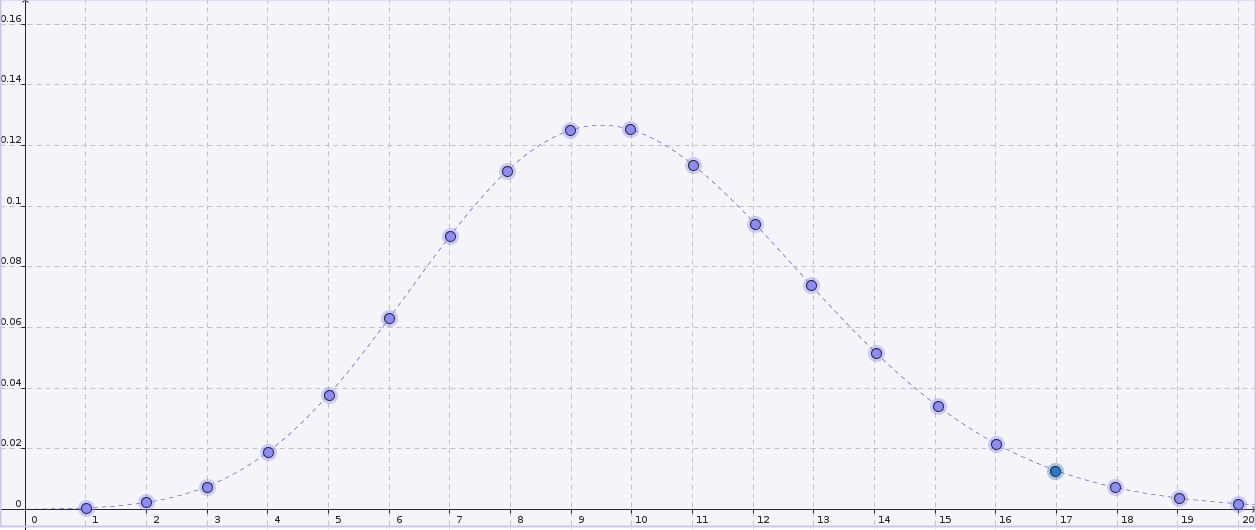
\includegraphics[width=15cm]{Cap1-Probabilidad/img/poisson.png}
        \caption{Gráfica de la probabilidad de que en determinado tiempo haya "x" bacterias $cm^2$ de cultivo cuando la tasa media es $10$.}
    \end{figure}
\end{Ejm}
Esta distribución es una de las más importantes de una variable discreta. Sus principales aplicaciones hacen referencia a la modelización de situaciones en las que nos interesa determinar el número de hechos de cierto tipo que se pueden producir en un intervalo de tiempo o de espacio, bajo presupuestos de aleatoriedad y ciertas circunstancias restrictivas.\\
Esta distribución se puede hacer derivar de un proceso experimental de observación en el que tengamos las siguientes características.
\begin{itemize}
    \item El experimento debe ser aleatorio.
    \item Se observa el experimento durante un cierto periodo de tiempo o a lo largo de un espacio de observación.
    \item La probabilidad de que se produzcan un número $n$ de éxitos en un intervalo de amplitud $t$ no depende del origen del intervalo (aunque, sí de su amplitud).
    \item La probabilidad de que ocurra un hecho en un intervalo infinitésimo es prácticamente proporcional a la amplitud del intervalo.
    \item La probabilidad de que se produzcan $2$ o más hechos en un intervalo infinitésimo es un infinitésimo de orden superior a dos.
\end{itemize}
Gracias a estas características podemos identificar cuando nos encontramos en el caso de una distribución de Poisson. \\\\
%%%%%%%%%%%%%%%%%%%%%% DISTRIBUCIÓN BINOMIAL %%%%%%%%%%%%%%%%%%%%%
Otra distribución sumamente útil es la binomial, para la cual primero será necesario definir la distribución de Bernoulli.\\ Esta distribución se define como aquel experimento aleatorio con únicamente dos posibles resultados, llamados genéricamente: éxito y fracaso.
Supondremos que las probabilidades de estos resultados son $p$ y $1-p$, respectivamente. Si se define la variable aleatoria $X$ como aquella función que lleva el resultado éxito al número $1$ y el resultado fracaso al número $0$, entonces decimos que $X$ tiene una distribución Bernoulli con parámetro $p\in[0,1]$.\\
Ahora, supongamos que efectuamos una serie de $n$  ensayos independientes Bernoulli en donde la probabilidad de éxito en cada ensayo es $p$. Si denotamos por $E$ el resultado éxito y $F$ el resultado fracaso, entonces el espacio muestral de este experimento consiste de todas las posibles sucesiones de longitud $n$ de caracteres $E$ y $F$ . Así el espacio muestral consiste de $2^n$ elementos. Si ahora definimos la variable aleatoria $X$ como aquella función que indica el número de éxitos en cada una de estas sucesiones, se tiene
\begin{eqnarray*}
    X(E E\ldots E)=n\\ X(FE\ldots E)=n-1\\ \vdots\\X(F F\ldots F)=0
\end{eqnarray*}
Notamos que $X$  puede tomar los valores $0,1,\ldots,n$  y esta variable aleatoria devolverá el número de éxitos al realizar un número determinado de experimentos. Analicemos esto con un ejemplo.
\begin{Ejm}
    Se realiza un experimento con un tipo de fertilizante orgánico para eliminar el musgo en una plantación. Se encontró una efectividad en los primeros experimentos del $75\%$.
    Si se aplica el mismo fertilizante en $3$ parcelas del mismo tamaño y bajo las mismas condiciones, esto nos dice que tenemos $3$ ensayos independientes Bernoulli con probabilidad de éxito de $p=0.75$  cada una.\\
    En esta situación nuestro espacio muestral es $$\Omega= \{E E E,\thinspace F E E,\thinspace E F E,\thinspace E E F,\thinspace F F E,\thinspace F E F,\thinspace E F F,\thinspace F F F\}$$
    Por ser independientes, la probabilidad de obtener que $2$ parcelas no pierdan su cosecha es preliminarmente,
    \begin{eqnarray}
        \label{eq-ejm-binomial-fertilizante}
    	p\thinspace p (1-p)=(0.75)^2(0.25)
    \end{eqnarray}
    Aquí hemos supuesto que en los  $2$ primeros ensayos resultaron exitosos, cuando ello no ocurrirá necesariamente así. Las diferentes formas en que los $2$ éxitos pueden distribuirse es de $3$ formas distintas $(F E E,\thinspace E F E,\thinspace E E F)$. (\ref{eq-ejm-binomial-fertilizante}) obtenemos la probabilidad que deseamos. $$3(0.75)^2(0.25)$$
\end{Ejm}

En general, las diferentes formas en que los $x$ éxitos pueden distribuirse en los $n$ ensayos está dada por el coeficiente binomial $n\choose x$. Al multiplicar este coeficiente binomial con el término $p^x(1-p)^{n-x}$ se obtiene la expresión de la función de probabilidad para la distribución binomial.
\begin{Def}
    Una variable aleatoria $X$ tiene una distribución binomial con parámetros $n$ y $p$ y se denota por $X\sim bin(n,p)$ si tiene por función de probabilidad
    $$f(x)=
    \begin{cases}
        {n \choose x} p^x(1-p)^{n-x}& x=0,1,\ldots,n\\0 & \textit{en otro caso}
    \end{cases}$$
\end{Def}
Un experimento se puede modelar con una distribución binomial si cumple que:
\begin{itemize}
    \item Sólo hay dos posibles sucesos resultantes del experimento:
    (éxito y fracaso).
    \item Las probabilidades de cada suceso son las mismas en cualquier realización del experimento ( $p$ y $1-p$ , respectivamente).
    \item Toda realización del experimento es independiente del resto.
\end{itemize}
Gracias a estas características podemos identificar cuando un experimento modela una distribución binomial.\\\\
%%%%%%%%%%%%%%%% DISTRIBUCIÓN EXPONENCIAL%%%%%%%%%%%%%%%%%%%%%%%%%%%%%%
\begin{Def}
    Decimos que una variable aleatoria continua $X$ tiene distribución exponencial con parámetro $\lambda>0$, cuando su función de densidad es
    $$\begin{cases}
        \lambda e^{-\lambda x}, & \mbox{si $x>0$}\\
        0, & \mbox{en otro caso}
    \end{cases}
    $$
\end{Def}
Se trata pues de una variable aleatoria continua con conjunto de valores en el intervalo $[0,\infty)$. Esta distribución se usa para modelar tiempos de espera para la ocurrencia de un cierto evento.\\
A pesar de la sencillez analítica de sus funciones de definición, la distribución exponencial tiene una gran utilidad práctica ya que podemos considerarla como un modelo adecuado para la distribución de probabilidad del tiempo de espera entre dos hechos que sigan un proceso de Poisson.\\
Tiene una gran utilidad en los siguientes casos:
\begin{itemize}
    \item Distribución del tiempo de espera entre sucesos de un proceso de Poisson.
    \item Distribución del tiempo que transcurre hasta que se produce un fallo, si se cumple la condición que la probabilidad de producirse un fallo en un instante no depende del tiempo transcurrido.
\end{itemize}
%%%%%%%%%%%%%%%%%%%%
Existen muchas más distribuciones recurrentes para variables aleatorias discretas, pero las mencionadas serán de nuestro principal interés.